% Please use the review version when submitting papers for review.
% The option below provides the final form of your paper

%\documentclass[review,article]{ij4uq}      %  review version
\documentclass[article]{ij4uq}              %  final version
% Use option "equation" for numbering equation as section

%\count0=115

% Added by author
\usepackage{graphicx}
\usepackage{caption}
\usepackage{subcaption}
\usepackage{stfloats}
\usepackage{fixltx2e}
\usepackage{placeins}

% \newcommand{\thesubfigure} [\alph{subfigure}]


%\fancypagestyle{plain}{%
%  \fancyhf{}
%  \fancyhead[R]{\small {\it DynaSearch User's Manual}, 1(1):xxx--xxx, \myyear\today}
%  \fancyfoot[R]{\vspace*{10pt}\small\bf\thepage }
%  \fancyfoot[L]{\fottitle}
%  }


\begin{document}

\volume{Volume 1, Number 1, \myyear\today}
\title{DynaSearch User's Manual}
\titlehead{DynaSearch User's Manual}
\authorhead{Cox, Malloy, House, \& Lindell}

% For authors with the same post address, uncomment the following
% 7 lines

\corrauthor[1]{Jonathan Cox}
\author[1]{Chris Malloy}
\author[1]{Jordan Gestring}
\author[1]{Donald House}
\author[2]{Michael Lindell}
\corremail{jlcox@g.clemson.edu}
\corrurl{http://www.clemson.edu/ces/savage/}
\address[1]{ School of Computing, 100 McAdams Hall, Clemson University, Clemson, SC 29634-0974, USA}
\address[2]{Hazard Reduction \& Recovery Center, College of Architecture, Texas A\&M University, College Station, TX 77843-3137, USA}

% End commands for all authors with the same address

% For at least 2 authors with different addresses, use instead the following commands

%\author[1]{Xiang Ma}
%\email{xm25@cornell.edu}
%\author[2]{James Taylor}
%\email{taylor@cornell.edu}
%\corrauthor[2]{Nicholas Zabaras}
%\corremail{zabaras@cornell.edu}
%\corrurl{http://mpdc.mae.cornell.edu/}
%\address[1]{Materials Process Design and Control Laboratory, Sibley School of Mechanical and Aerospace
%Engineering, 101 Frank H.T. Rhodes Hall, Cornell University, Ithaca, NY 14853-3801, USA}
%\address[2]{Another Address Here,   Cornell University, Ithaca, NY 14853-3801, USA}

% End information for at least 2 authors with different addresses


\dataO{\mydate\today}
%\dataO{}
\dataF{\mydate\today}
%\dataF{}

\abstract{
}

% Up to seven key words are required. Please provide a list consulting
% the keywords given in the document IJ4UQ-KeyWords.pdf if different
% key words as needed.

\keywords{Experiment Design}


\maketitle




\section{Introduction}

DynaSearch is a web based system that allows the end user to create and run a variety of user studies.  The basic toolset supports the construction of studies designed to test how users collect and process information by recording the order and duration of mouse clicks on a set of pre-designed page elements, such as text boxes.  In addition, DynaSearch supports more complex user studies by allowing end users to write and embedd their own custom experiements through the use of Java Applets, HTLM5, WebGL, and D3.  The rest of this document will explain these tools in greater detail, but in order to provide you with a picture of the end product, a short example of what can be created is detailed below.

\subsection{A Short Example}

\subsubsection{The Login Screen}

\begin{figure}[h!]
 \centering
 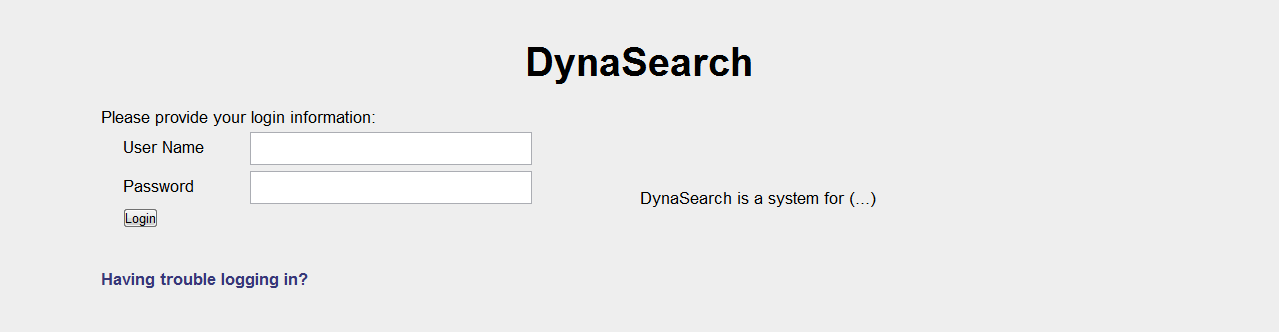
\includegraphics[width=4.0in]{figures/login.png}
 \caption{Users will start an experiment by logging into the DynaSearch system through the login screen.}
 \label{fig:login}
\end{figure}
\FloatBarrier

All users should be provided with a user name and password so that they may login to the system. The login screen is displayed in \ref{fig:login}.

\subsubsection{The Size Registration Screen}

\begin{figure}[h!]
 \centering
 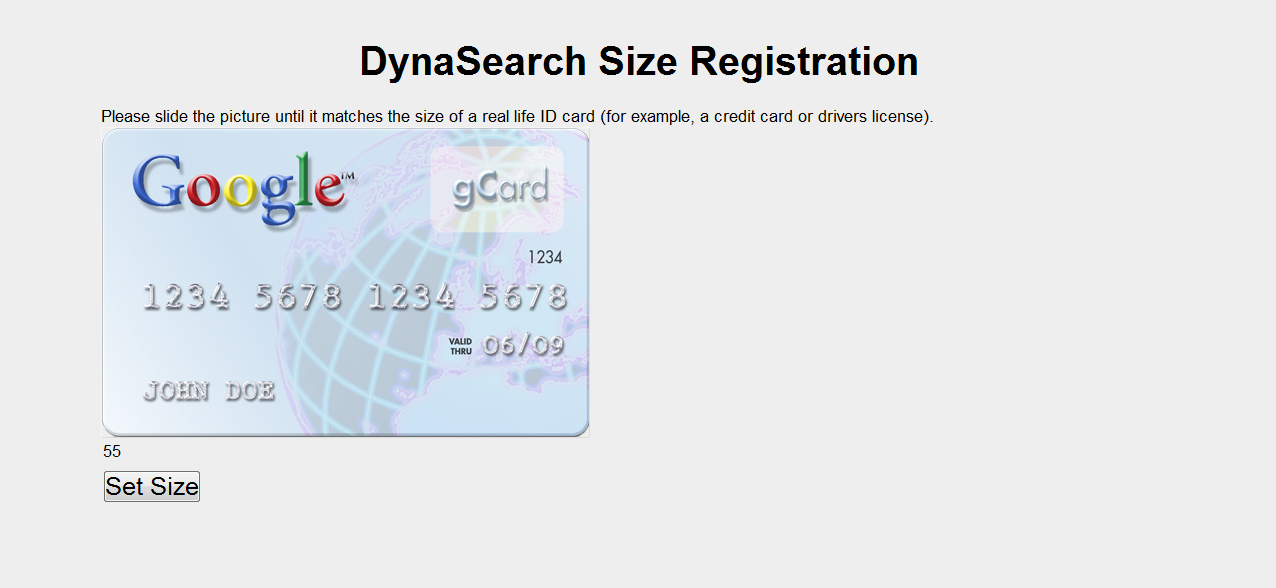
\includegraphics[width=4.0in]{figures/size_reg.png}
 \caption{Users must first register the size of their screen.}
 \label{fig:sizereg}
\end{figure}
\FloatBarrier


In order to ensure that all users see screen elements of the exact same size, regardless of screen size and resolution, a size registration must first be performed. This is done by holding a physical credit card up to the screen and sliding the edges of the Google credit card image until it is the same size as the physical card. This screen is shown in \ref{fig:sizereg}.

\subsubsection{The Instruction Screen}

\begin{figure}[h!]
 \centering
 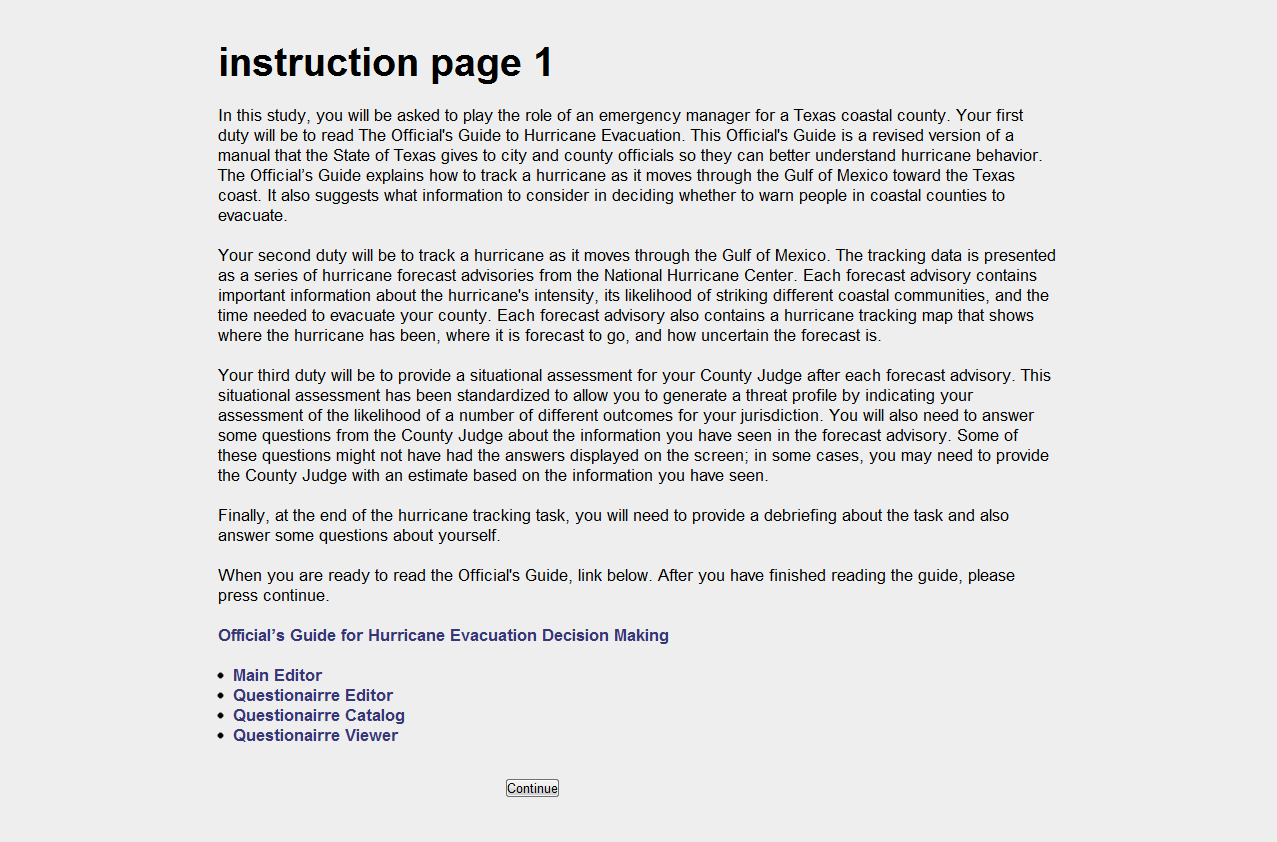
\includegraphics[width=4.0in]{figures/instruction_page.png}
 \caption{The instruction screen displays information for the users.}
 \label{fig:inst}
\end{figure}
\FloatBarrier

Users can be supplied with supplemental information using the instruction screen. A sample instruction screen is displayed in \ref{fig:inst}. 

\subsubsection{The Training Screen}

\begin{figure}[h!]
 \centering
 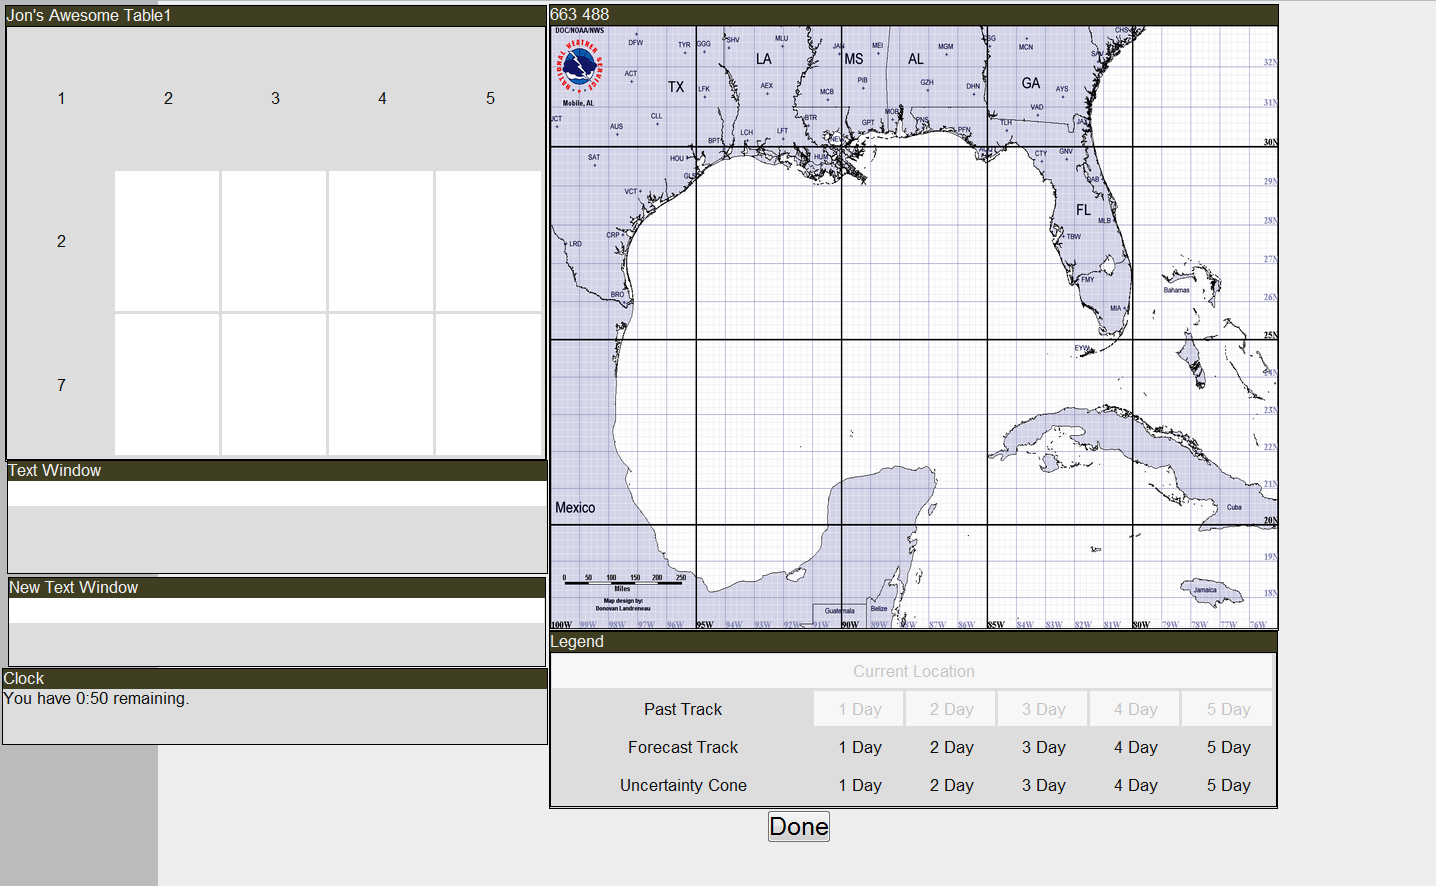
\includegraphics[width=4.0in]{figures/training_page.png}
 \caption{The training screen records information based on user clicks.}
 \label{fig:train}
\end{figure}
\FloatBarrier

The training screen records the order and duration of participant clicks. The participant clicks on the screen in order to uncover certain pieces of information, whether it is a cell of a table or information drawn over an image. A sample training screen is displayed in \ref{fig:train}.  Training screens can include a timer which will force participants to move to the next portion of the experiment after a defined period of time.  Training screens also support embedded Java applets, HTML 5 pages that utilize WebGL, and D3.  This will be explained in greater detail in the section of the manual that covers building training pages.

\subsubsection{The Survey Screen}

\begin{figure}[h!]
 \centering
 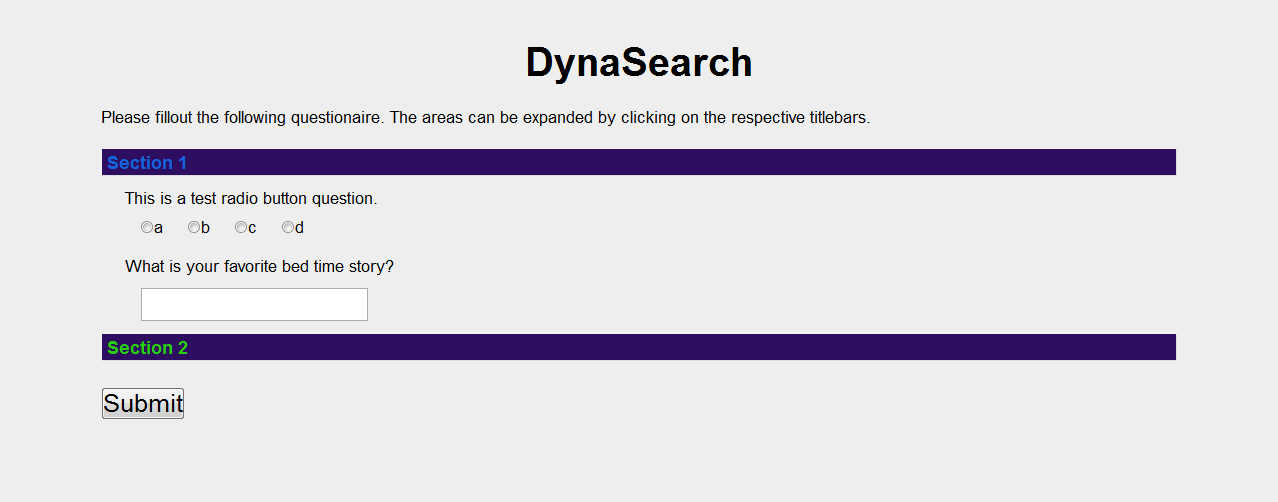
\includegraphics[width=5.0in]{figures/survey_page.png}
 \caption{The survey screen allows the users to answer specific questions.}
 \label{fig:survey}
\end{figure}
\FloatBarrier

The survey screen allows the participants to respond to specific questions designed by the end user. There are currently two question types available for use.  These are radio button questions and free response questions.  In addition, frequently used questions can be stored and inserted into questionnaires as needed.  A sample survey screen is displayed in \ref{fig:survey}.

\subsubsection{Complete Example}


%% \section{Introduction} %for journal use above \firstsection{..} instead

\section{Administrative Tools}

\subsection{A Quick Overview}
From this point forward, the "you" will refer to the individual creating the experiments, and "user" refers to the research participants. 

The DynaSearch system allows for the creation of user studies that can be composed of three different types of pages. The first is the instruction page. Here, basic HTML is displayed that can be used to convey specific instructions to users or as a means of supplying them with supplemental information. The second is the training page. This page can be composed of text boxes, tables, and images that are all hidden on the page's initial load.  In order for users to see hidden information and interact with any of these elements, they must click on it. The order and duration of these clicks is tracked by a database typically hosted on the web server. The training page can also house custom applets that offer a wider variety of interactions.  The last type of page is a questionnaire which allows users the opportunity to provide feedback.  Additionally, it can serve as a way to test the users on previously displayed information.

Accounts with administrator access are given access to the \textbf{Administrator's Page} where links to the different editors are listed. Instruction pages, training pages, and questionnaire pages can be created in any order. The survey creation tool defines an experiement by linking pages together, and should not be used until all of the pages for a given experiment have been completed.

The remainder of this section will explain the use and operation of these editors. For more information regarding the database, please refer to Appendix A. For more information on the file system, please see Appendix B.

\subsubsection{Instruction Pages}
To create an instruction page, just create a text file that contains the information desired and place it in the \newline \texttt{DynaSearch/expResources/instructPages/} directory located in the DynaSearch file system. Because this data will be inserted between the $<\texttt{body}>$ tags of the template instruction page, any additional HTML tags and scripting maybe used as desired. These files will automatically be available from the Survey Setup editor page. 

\subsubsection{Training Pages}

\begin{figure}[h!]
 \centering
 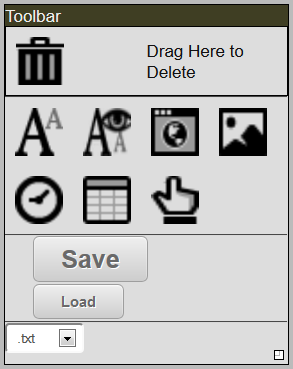
\includegraphics[width=2.0in]{figures/toolbar.png}
 \caption{The icons represent the trash bin, text window, visible text window, applet window, image window, clock, table window, interactive table window, and legend window respectively.}
 \label{fig:tool}
\end{figure}
\FloatBarrier

To access the training page, select the \textbf{Training Page Editor} link from the \textbf{Administrator's Page}. This will take you to a blank training editor page with the toolbar window located in the upper left window. With the exception of the trash can, each of the icons on the toolbar allow for the creation of a different window. The toolbar window is displayed in \ref{fig:tool}. The toolbar window and any other created window can be moved by clicking and dragging on the title handle of the window.

\paragraph{The Trash Bin}

The Trash Bin allows you to delete unwanted windows. Simply click on the title bar of the window you wish to remove, and drag it over the trash can. When you release it, it will be deleted.

\paragraph{The Text Window}
The Text Window is used to display paragraphs or sections of text to the user. These will be hidden during a user study until the user clicks on the section containing the text. The title of the window and the text inside can both be modified by clicking on the blue icon in the top right corner of the window. It can be resized by clicking and dragging on the white box in the bottom right corner of the window.

\paragraph{The Visible Text Window}
The Visible Text Window is similar to the Text Window, with the exception that the text will always be visible to users.  The contents will not be hidden during the course of a user study.

\begin{figure}[h!]
 \centering
 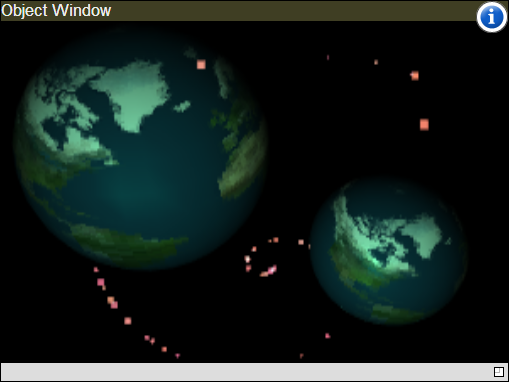
\includegraphics[width=4.0in]{figures/webgl.png}
 \caption{The Applet Window will let you embed various scripts and applets to extend the user study.}
 \label{fig:webgl}
\end{figure}
\FloatBarrier

\paragraph{The Applet Window}
The Applet Window lets you embed Java applets as well as HTML5 and JavaScript code that can include WebGL or D3 scripts into the Training Page.  To assign an applet, HTML5, or JavaScript file to the Applet Window, click on the blue icon in the top right corner of the window and provide the file name in the prompt that appears.  The files should be stored in the \texttt{DynaSearch/assets/userObjects/} directory located in the DynaSearch file system.  An example of the Applet Window can be seen in \ref{fig:webgl}.


\paragraph{The Image Window}
The Image Window allows you to display a static image.  The chosen image will always be displayed unless a Legend Window is associated with with it.  Please see the section covering the Legend Window for more information.  To select the image to be displayed, click on the blue icon in the top right corner of the window and provide the file name in the prompt that appears.   The files should be stored in the \texttt{DynaSearch/assets/images/} directory located in the DynaSearch file system.

\paragraph{The Clock Window}
The clock window determines how long a page will be available to a user. By clicking on the blue icon, you can specify the number of minutes that each user should receive. The default time is 20 minutes. If no clock window is created, then the window will be available to the user until they click on the Done button. Please note that the clock window will not actually be displayed while the experiment is being run.

\begin{figure}[h!]
 \centering
 \begin{subfigure}[b]{0.4\textwidth}
    \centering
    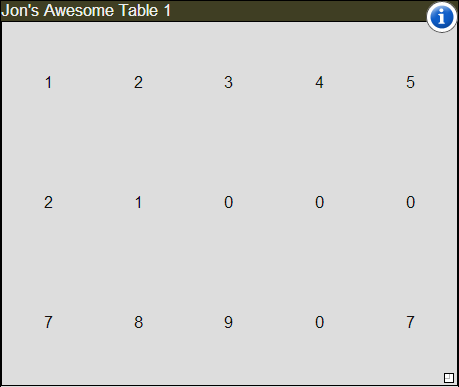
\includegraphics[width=2.0in]{figures/table_uncovered.png}
    \caption{In training page editor}
    \label{fig:tableUN}
 \end{subfigure}
 \begin{subfigure}[b]{0.4\textwidth}
    \centering
    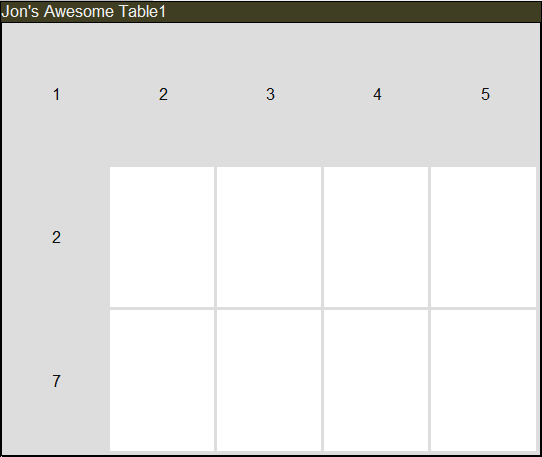
\includegraphics[width=2.0in]{figures/table_covered.png}
    \caption{Durring user study}
    \label{fig:tableCV}
 \end{subfigure}
 \caption{Table Window}
 \label{fig:tableWindow}
\end{figure}

%\begin{figure}[]
 %\centering
 %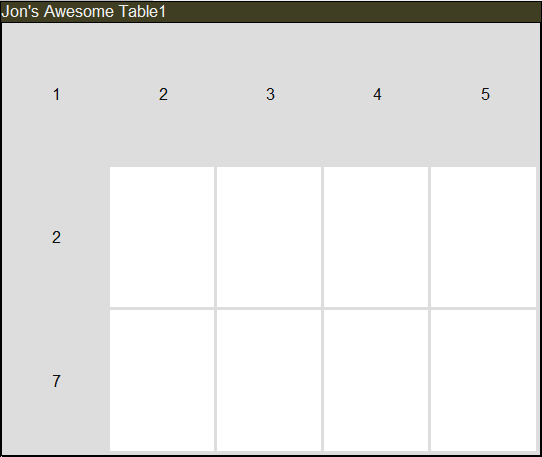
\includegraphics[width=2.0in]{figures/table_covered.png}
 %\caption{Table Window Covered}
 %\label{fig:table_cv}
%\end{figure}
\FloatBarrier

\paragraph{The Interactive Table Window}

The Interactive Table Window displays information in a table format, as demonstrated in \ref{fig:tableWindow}.  The first row and column will always be visible, while the other fields will be covered by a white box.  When clicked, the box will become transparent, allowing users to see the data values underneath.  Clicking on the blue icon will allow the user to change both the table name and the file in which the table data is stored. These text files are stored in the directory \texttt{DynaSearch/expResources/tables}.  Columns are separated by commas, and the rows are separated by new lines. To resize the table, click and drag on the white box in the bottom right corner of the table window. You must resize the table manually in order to test that the information contained is displayed correctly.

In order to distinguish which table a user is clicking on from the entries in the database, the tables in an experiment should have unique table names.

\paragraph{The Table Window}

The Table Window behaves in the same manner as the Interactive Table Window with the exception that the data is visible at all times during the course of a user study.  Because of this, no click data is recorded for this type of table.

\paragraph{Loading A Training Page}
To load a previously saved training screen, pick the training file from the drop down menu that you wish to work with and hit the Load button. Note that to save any changes made to this training screen, you must hit the Save button before navigating away from the page.

\paragraph{Saving A Training Page}
The Save button will prompt you to enter a name to save the file as. The extension .txt will automatically be added to the name you supply, so it is not necessary to include that in the file name. For example, if you want the file name to be test1.txt, enter only test1.

\subsubsection {Questionnaire Editor}

\begin{figure}[h!]
 \centering
 
\includegraphics[width=5.0in]{figures/place.eps}
 \caption{Questionnaire Toolbar}
 \label{fig:questTool}
\end{figure}
\FloatBarrier

The Questionnaire Editor allows you to create a questionnaire that can be taken by users as they progress through an experiment. There are five basic building blocks that can be incorporated into each type of questionnaire, four of which are accessed through the toolbar displayed in \ref{fig:questTool} and the last of which is selected from the drop down menu on the page. Each of these is described in greater detail below. 
The information submitted by the users is kept in a file with the same name as the user's id, and is stored in the directory DynaSearch/userData. For more information on the file system, please refer to Appendix B.

\paragraph{Section}

The Section option allows you to split the questionnaire into different sections. Only one questionnaire section is open at a time. Each section is accessed by clicking on the section header bar. Note that this will only be visible to the user. The questionnaire will remain expanded while in administrator mode. 
To create a section header, click on the Section radio button, and then hit Next.A prompt for the title will appear. After you enter a title and select the Next button, the section header will be visible on the page. To remove a section header, simply click on the red minus symbol above the upper right corner of the element.

\paragraph{Radio Buttion Question}
To create a radio button question, select the Radio Button Question option from the toolbar and hit Next. DynaSearch will display a prompt for the question as well as the number of radio button choices. After you fill this information out and again hit the Next button, DynaSearch will prompt you to provide the specific value for each radio button option. 
Note that DynaSearch will record the information as the index value you choose, and not the value you enter. To remove a radio button, simply click on the red minus symbol above the upper right corner of the element.

\paragraph{Text Question}
The Text Question option allows for the creation of a free response question. By selecting this option and clicking on the Next button, you will be prompted to provide the question for the text, as well as the number of characters that should be displayed on the screen for a response. Please note that the user may enter a response that is larger than this value, and that the entire response will be saved. This number only dictates how much of the response is displayed on the screen at one time. 
After this information is filled out, the question can be added to the screen by hitting the Next button. To remove a text question, simply click on the red minus symbol above the upper right corner of the element.

\paragraph{Line of Text}
The Line of Text option allows you to provide users with additional instructions or information. After selecting this option and hitting the Next button, DynaSearch will prompt you to enter in the text that should be displayed. To add the information to the page, click the Next button again. To remove a line of text, simply click on the red minus symbol above the upper right corner of the element. 

\paragraph{Drop Down Question List}
The administrator may place a prewritten radio or text question from the Questionnaire Catalog by selecting the appropriate question designator from the drop down menu on the page. For more information regarding the Questionnaire Catalog, please see the appropriate section of this guide. To remove a question added by the drop down list, simply click on the red minus symbol above the right corner of the element. 

\paragraph{Save}
To save a questionnaire, hit the Save button. DynaSearch will prompt you to create a title for the questionnaire at the bottom of the page. After you enter the title, click the Save button on the bottom of the page.

\subsubsection{Questionnaire Catalog}

\begin{figure}[h!]
 \centering
 
\includegraphics[width=5.0in]{figures/place.eps}
 \caption{Questionnaire Catalog Toolbar}
 \label{fig:questCatTool}
\end{figure}
\FloatBarrier

The Questionnaire Catalog can be used to create questions that will be used multiple times throughout several questionnaires. You can create two question types from this screen through the toolbar shown in \ref{fig:questCatTool}. They are the radio question and text question types.

\paragraph{Radio Button Question}
To create a radio button question, select the Radio Button Question option from the toolbar and hit Next. DynaSearch will display a prompt for the question as well as the number of radio button choices. After you fill this information out and again hit the Next button, DynaSearch will prompt you to provide the specific values for each radio button option. 
After you fill the values, hit Next to save the question. A text box on the page will appear where a question designator can be created. This will be used to identify the question from the Question Editor screen via the Drop Down Question List. 
Note that DynaSearch will record the information as the index value you choose, and not the value you enter.

\paragraph{Text Question}
The Text Question option allows for the creation of a free response question. By se.lecting this option and clicking on the Next button, you will be prompted to provide the question for the text, as well as the number of characters that should be displayed on the screen for a response. Please note that the user may enter a response that is larger than this value, and that the entire response will be saved. This number only dictates how much of the response is displayed on the screen at one time. 
After you fill this information out and again hit the Next button, DynaSearch will prompt you to provide the specific values for each radio button option. After you fill the values, hit Next to save the question. A text box on the page will appear where a question designator can be created. This will be used to identify the question from the Question Editor screen via the Drop Down Question List.

\subsubsection{Questionnaire Viewer}
You can use this screen to view previously created questionnaires. To view a questionnaire, select the questionnaire from the drop down list, and click the Load button. 
It is important to note that once a questionnaire is saved in the Questionnaire Editor, it can not be reloaded and changed in anyway without accessing the saved questionnaire directly in the sur questions database table and modifying the Value field. However, it can be completely overwritten by a new questionnaire.

\subsubsection{Experiment Editor}

\begin{figure}[h!]
 \centering
 
\includegraphics[width=5.0in]{figures/place.eps}
 \caption{Experiment Editor Interface}
 \label{fig:eeInterface}
\end{figure}
\FloatBarrier

The Experiment Editor allows you to combine any number of instruction pages, train.ing pages, and questionnaires into a single experiment. The interface shown in \ref{fig:eeInterface} will allow you to select and assemble the various elements required. To change the title of a new experiment, click on the current title. It is located at the top of the screen and is surrounded by quotes with a default value of, "New Experiment".

\paragraph{Add Information Page}

\begin{figure}[h!]
 \centering
 
\includegraphics[width=5.0in]{figures/place.eps}
 \caption{Information Page Inserted}
 \label{fig:infoInsert}
\end{figure}
\FloatBarrier

The Add Information Page button will allow you to insert a new information page into the current experiment. When this button is clicked, a new page is inserted into the current list of pages, as is shown in \ref{fig:infoInsert}. The default title of the page is New Page. You can modify this by clicking on the current title, at which point DynaSearch will prompt you to enter a new one. The default file associated with this page is set to (unassigned), which can also be changed by clicking on it. Please be sure to enter the full file name of the instruction page that you wish to use. A list of the currently available instruction pages can be found by selecting the drop down list entitled Active Instruction Pages. The files listed are those that are stored in the DynaSearch/expResources/instructPages directory.

To change the sequence of a page, click and drag the blue box on the left hand side of the pageÕs label up or down to slide it into the desired location. To remove a page from your list of pages, select the red minus sign on the right hand side of its label.

\paragraph{Add Training Page}

\begin{figure}[h!]
 \centering
 
\includegraphics[width=5.0in]{figures/place.eps}
 \caption{Training Page Inserted}
 \label{fig:trainInsert}
\end{figure}
\FloatBarrier

The Add Training Page button will allow you to insert a new training page into the cur.rent experiment. When this button is clicked, a new training page is inserted into the current list of pages, as is shown in \ref{fig:trainInsert}. The default title of the page is New Page. You can modify this by clicking on the current title, at which point DynaSearch will prompt you to enter a new one. The default file associated with this page is set to (unas.signed), which can also be changed by clicking on it. Please be sure to enter the full file name of the training page that you wish to use. A list of the currently available training pages can be found by examining the drop down list entitled Active Advisories. The files listed are those that are stored in the DynaSearch/expResources/advisory directory.

To change the sequence of a page, click and drag the blue box on the left hand side of the pageÕs label up or down to slide it into the desired location. To remove a page from your list of pages, select the red minus sign on the right hand side of its label.

\paragraph{Add Survey Page}

\begin{figure}[h!]
 \centering
 
\includegraphics[width=5.0in]{figures/place.eps}
 \caption{Survey Page Inserted}
 \label{fig:surveyInsert}
\end{figure}
\FloatBarrier

The Add Survey Page button will allow you to insert a new questionnaire into the cur.rent experiment. When this button is clicked, a new survey page is inserted into the current list of pages, as is shown in \ref{fig:surveyInsert}. The default title of the page is New Page. You can modify this by clicking on the current title, at which point DynaSearch will prompt you to enter a new one. The second parameter is the file name. Its default value is listed as (unassigned). This is the name of the file that the questionnaire will be saved to in the experimentÕs directory. The extension of any filename given should be .txt.

The final parameter in the list is the name of the questionnaire that you would like to use. This should be the name of the saved questionnaire that was created using the Questionnaire Editor. A list of all of the available questionnaires is under the drop down listed entitled Active Surveys. 
To change the sequence of a page, click and drag the blue box on the left hand side of the pageÕs label up or down to slide it into the desired location. To remove a page from your list of pages, select the red minus sign on the right hand side of its label.

\paragraph{New Survey}
To start a new survey, click on the New Survey. Doing this will clear any work that has been done, so it is important to save previous work before continuing.

\paragraph{Save Survey}
To save a survey that you have been working on, click on the Save Survey button. DynaSearch will then use the experiment name and automatically create a folder in the directory DynaSearch/hurricane data. This is explained in greater detail in Appendix B.

\paragraph{Load Survey}
To load a previously saved survey, select the survey that you wish to load from the drop down menu and then click on the Load button. 
Appendix A.

\section{Appendix A: Database Information}
The tables listed below are used for the DynaSearch system. Any other tables you find in the database are legacy items from the original EMDSS application on which this website was based. The tables have no dependency on each other. Because of this, the resulting structure is very simple and easy to maintain. The tables are explained in greater detail below. The database used for DynaSearch is MySQL 5.1. The entire system was built using version 2.0 of wampServer.

\subsection{sur clicks}
The sur clicks table records the click information for each user on training pages. Each entry in the database represents a single click. Each individual field is explained below. 

\subparagraph{Dummy}
This is the primary key for the entry. It allows you to determine when an element was inserted into the table in relation to the other elements. This can be useful for reordering the elements after ordering them by another value.

\subparagraph{UserName}
This is the user name of the individual that did the click.

\subparagraph{SessionNumber}
This field was placed to keep track of users between separate experiments. It was determined that it would not be of much help for the currently designed experiments and so was never fully implemented. It has been left for possible future expansion of the software. For now it is assumed that each user only participates in one experiment once. If this is not the case, then their data will need to be cleared out of this table beforehand and their position number will need to be reset in t user.

\subparagraph{ObjClicked}
This is the item that was clicked on a particular training page. Every objects name begins with "x toTrack". From there the naming convention differs, depending on the element in question. The details for each of the three element types are given below.
 
\emph{Tables}
The format for tables is: x toTrackTable "file name" "table name" "row" "column". So for example, if the file name was testFile.txt, the table name was Table 1, and the user clicked on the first row with the second column, then the entry would be x toTrackTable testFile.txt Table1 1 2. 
It is important to note that for any given experiment, there should be no two tables that share both the same file name and table name. Otherwise, it will be impossible to distinguish between them in the database.

\emph{Map Legends}
The format for map legends is: x toTrackTable mapLegend adv "advisory number" "row" "column". So for exam.ple, if the advisory number for the map on the training screen was five and the user clicked on the second row and the third column, then the entry would be x toTrackTable mapLegend adv 5 2 3). 
It is important to note that no two maps should have the same advisory number for a given experiment. Otherwise, it will be impossible to distinguish between them in the database.

\emph{Text Blocks}
The format for text blocks is: x toTrackText "window name". So for example, the the name of the text window was "Advisory Information", then the entry would be x toTrackText AdvisoryInformation. 
It is important to note that no two text blocks should have the same title throughout an experiment. Otherwise, it will be impossible to distinguish between them in the database.

\subparagraph{ClickLength}
This gives how long the element was clicked in seconds.

\subparagraph{ClickNumber}
This gives the order that an element was clicked on a specific training page. Ordering the elements by their Dummy value will return the sequence in which the elements of a single training page were accessed.

\subsection{sur question}
This table holds all of the questionnaires that have been created within DynaSearch. Everything in this database is handled internally, so it should almost never need to be accessed. It should be noted that once experiments are created, the information in the Value field is copied to a file in the file system. This is designed to protect individual experiments from issues that may occur with the database. The details of each field are given below.

\subparagraph{id}
The id field serves as the primary key for an entry. It should never need to be referenced. 

\subparagraph{Name}
This is the name of the given questionnaire. It is what is displayed when trying to insert the questionnaire into different experiments. Each should be unique. 

\subparagraph{Value}
This is the HTML that makes up the questionnaire. It is stored in its basic format. If the questionnaire needs to be edited in any way after it is saved, it will have to be through this field, as there is currently no way to modify pre-existing surveys. 

\subsection{sur randquestion}
This tables holds the questions that are created through the Questionnaire Catalog. They are single questions that maybe repeatedly inserted into a questionnaire. The details of each field are given below. 

\subparagraph{id}
The id field serves as the primary key for an entry. It should never need to be referenced. 

\subparagraph{Designator}
This is how the question is identified from the Questionnaire Editor. These should be unique values. 

\subparagraph{Value}
This is the HTML that makes up the question, and is stored in its basic format. If the question needs to be modified in anyway after it is saved, it will have to be through this field, as there is currently no way to change a question once it has been saved. 


\subsection{t experiments }
The experiments table holds all of the information that is saved from the Experiment Editor. Short of removing experiments from the database, this table should rarely be referenced. 

\subparagraph{id} 
The id field serves as the primary key for an entry. It should never need to be referenced. 

\subparagraph{ExperimentShortName}
The experiment short name is the name of the experiment that will be seen from the Experiment Editor. It will be the name given to the experiment on creation without any spaces or special characters. 

\subparagraph{ExperimentString}
This field contains a string which represent the experiment referenced. Most of it is stored in hexadecimal characters, and is therefore unreadable by itself. This informa.tion should only ever be accessed through the Experiment Editor. This string keeps track of the order of the pages, as well as the names of the files that correspond to each page in the experimentÕs folder. 


\subsection{t user}
This table holds all of the account information for a given user. A detailed look at the fields is given below.

\subparagraph{User ID}
This is the identification that the user provides to the login screen in order to access the experiment. 

\subparagraph{County ID}
Lists the current county of the user. This field is currently not used. 

\subparagraph{UPassword}
The password for the user. Because the system was designed for academic purposes and no personal information is being stored, these passwords are not encrypted in any.way.

\subparagraph{User Type}
This specifies the role of the account. An "A" designates the account as an adminis.trator. If this is true, they will automatically taken to the administrator page on login. A "U" designates the account as user. On login this individual will be taken to the experiment they are participating in. They should not have access to any of the editors or administrator page. 

\subparagraph{Name}
Real name of the user. 

\subparagraph{scaleW}
This field only applies to users. It is the width measurement that is recorded from the size registration page, and is used to ensure that every element on a training page is displayed with proper proportion, regardless of the monitorÕs screen size or resolution. 

\subparagraph{scaleH}
This field only applies to users. It is the height measurement that is recorded from the size registration page, and is used to ensure that every element on a training page is displayed with proper proportion, regardless of the monitorÕs screen size or resolution. 

\subparagraph{current position}
This field only applies to users. It determines where in an experiment the user should be, should they log out and try to log back in before the completion of the experiment. It should also prevent users from trying to back track in an experiment, though this behavior may vary from browser to browser. 

\subparagraph{experiment}
This field only applies to users. It determines which experiment will be displayed for a user when they log into the system. The value must be one of the Experiment Short Name entries listed in the t experiments table. 

\subparagraph{FORECAST}
Determines whether or not the user should be able to click on the row of forecast buttons in the map legend window. A value of 0 means that the user will not be able to access this information, while a value of 1 means that they will. 

\subparagraph{PAST TRACK}
Determines whether or not the user should be able to click on the row of past track buttons in the map legend window. A value of 0 means that the user will not be able to access this information, while a value of 1 means that they will. 

\subparagraph{CONE}
Determines whether or not the user should be able to click on the row of cone of uncertainty buttons in the map legend window. A value of 0 means that the user will not be able to access this information, while a value of 1 means that they will. 

\subparagraph{CURRENT}
Determines whether or not the user should be able to click on the current location button in the map legend window. A value of 0 means that the user will not be able to access this information, while a value of 1 means that they will.

\section{Appendix B: Filesystem Information}
The file system is separated into five sections. These are the main files, experiment files, experiment resources, user data, and other assets. Each of these is detailed below.

\subsection{Main Files}
The main DynaSearch directory contains the files that are used during interaction with and creation of experiments. A quick overview is given of the most notable files.

\paragraph{admin.php} - The page that administrators login to

\paragraph{advance.php and director.php} - These files interact to ensure that users go to the right page when they login and click through the experiment

\paragraph{dynaview.php} - The main training page that users interact with

\paragraph{editor.php} - This is the page where the Training Page Editor loads

\paragraph{instructions.php} -This is the page that is used to display instructions to the users 

\paragraph{questDisplay.php} -This page is used to implement the Questionnaire Viewer

\paragraph{questEditor.php} -This page is used to implement the Questionnaire Editor 

\paragraph{question.php} -This page is used to display questionnaires to users 

\paragraph{randQuestEditor.php} -This page is used to implement the Questionnaire Catalog 

\paragraph{survey setup.php} -This page is used to implement the Experiment Editor

\subsection{Experiment Files}
Inside the directory DynaSearch/hurricane data is a folder for every experi.ment that has been created. Inside these folders are files that correspond to each of the pages of the experiment. This means that for each instruction page, each training page, and each questionnaire, there will be one file in the experiment's folder that cor.responds to it. Instruction and questionnaire pages will be displayed as HTML, while the training pages are encoded as hexadecimal characters.

\subsection{Experiment Resources}
The folder DynaSearch/expResources contains a number of sub-folders which store the information needed to create the various instruction and training pages. The purpose of these folders is detailed below.

\paragraph{advisory}
This directory contains a copy of all of the training pages that have been created. The contents are displayed in hexadecimal characters, and are only utilized inside the Dy.naSearch framework.

\paragraph{images}
This directory contains copies of all the images that can be used in the training pages, along with files that contain the geographic information for each image.

\paragraph{instructPages}
This directory contains all of the instruction pages that can be used in an experiment. Though they all have the .txt extension, the contents are just the HTML that would be found between the <body> tags in a standard HTML file. 

\paragraph{tables}
This directory contains all of the files containing table information which can be used in the training pages.

\paragraph{tracking}
This directory contains all of the files that hold hurricane tracking information which can be used in the training pages.

\subsection{User Data}
This folder holds the user responses for each survey that a user participates in, as well as their window scaling information. Every value is comma separated, and commas that users type in the free response questions are replaced with a '. The files are named according to the user's user name.

\subsection{Other Assets}
The DynaSearch/assets directory hold all of the background scripts and files that are used to make the DynaSearch system work. Below is a list of the subdirectories and any major files that are located in each.

\paragraph{images}
This directory holds all of the images utilized by DynaSearch.

\paragraph{php}
This directory holds all of the php files that are used behind the scenes.

\subparagraph{config.php} -Holds the database information that is required to access and modify data 

\subparagraph{standard.php} -Holds the standard header information for every php file. This includes the <head> tags. 
	
\subparagraph{db util.php} -Provides the connection to the database specified in config.php

\paragraph{scripts}
This directory holds all of the javascript files that are used in DynaSearch. There are a few notables files. 

\subparagraph{editor.js} -This is a rather large file that stores all of the functions used by the Training Page Editor and also by dynaview.php.
 	
\subparagraph{timer.js} -This file contains the scripts that are used to cover all of the elements on a training page, as well as to keep track of the user click information before it is sent to the server.

\paragraph{style}
This directory just holds the style information for DynaSearch.

\section{Appendix C: Installing Dynasearch}
To Install the DynaSearch Software:

1. Copy the DynaSearch folder to the appropriate folder utilized by the web server. 

2. Go the the Þle DynaSearch/assets/php/config.php and provide the 
appropriate information for the following: 


\emph{DB HOST} -this is the host name where the database is located
	
\emph{DB USER} -this is the administrator account that will be able to log in, query, and make changes to the EMDSS database
	
\emph{DB PASS} -this is the password for DB USER account
	
\emph{Note} -Do not change the database name unless the name is also changed 
on the database server 

3. Import the EMDSS database into the MySQL server. The database Þle is named EMDSS DB.sql.zip and can be found in the DynaSearch directory. 


4. To test whether the system was imported correctly, go to *webaddress*/DynaSearch/login.php with the user name jlcox5 with the password jlcox5. It should take you to a test.ing page. 

If there are any problems or questions, please contact: 
Jonathan Cox at jlcox@g.clemson.edu 
%% The Acknowledgements part is started with the command \acknowledgements;
%% acknowledgements are then done as normal sections before appendix
%% \acknowledgements

\acknowledgements

This work was supported in part by NSF and NOAA under grant NSF CHI 2008001386.


%% The Appendices part is started with the command \appendix;
%% appendix sections are then done as normal sections and after Acknowledgements
%% \appendix

%% \section{}
%% \label{}

%% References without bibTeX database:

%\begin{thebibliography}{-8}

%% \bibitem must have the following form:

%\small{
%\bibitem{key}

%...

%}

%\end{thebibliography}

%% References with bibTeX database:

\bibliographystyle{IJ4UQ_Bibliography_Style}

\bibliography{hurricane}
\end{document}
